\documentclass{article}
\usepackage[utf8]{inputenc}

% Basic packages
	\usepackage{amssymb}
	\usepackage{amsmath}
	\usepackage{graphicx}
	\usepackage[czech]{babel}
	\usepackage{natbib}

% Relevant packages
	\usepackage{bm}
	\usepackage{bbm}
	\usepackage{geometry}
	\usepackage{enumitem}
	\usepackage{listings}
	\usepackage{multicol,float}
	\usepackage{subcaption}

% Document settings
	\geometry{a4paper,margin=15mm}

	\setlist[itemize]{nolistsep,noitemsep}
		
	\setlength{\parindent}{0pt}
	\setlength{\parskip}{1.5em}
	\renewcommand{\baselinestretch}{1.2}

	\setlength{\abovedisplayskip}{1.2em}
	\setlength{\belowdisplayskip}{1.2em}
	\renewcommand{\arraystretch}{1.2}

\begin{document}
% \begin{multicols}{2}
	\section{Popište možné tvary dynamických systémů pro modely: spojité-diskrétní, lineární-nelineární. }
	
	\subsection*{Lineární spojitý systém v časové oblasti}
	\begin{align*}
		\bm{\dot{x}} &= \bm{A}\bm{x} + \bm{B}\bm{u} \\
		\bm{y} &= \bm{C}\bm{x} + \bm{D}\bm{u}
	\end{align*}
	\subsection*{Lineární spojitý systém ve frekvenční oblasti}
	\begin{align*}
		s\bm{x} &= \bm{A}\bm{x} + \bm{B}\bm{u} \\
		\bm{y} &= \bm{C}\bm{x} + \bm{D}\bm{u}
	\end{align*}
	Po úpravě $\bm{x}(s\bm{I} - \bm{A}) = \bm{B}\bm{u}$ můžeme dosadit
	\begin{equation}
		\bm{y} = \bm{C}(s\bm{I}-\bm{A})^{-1}\bm{B}\bm{u}+\bm{D}\bm{u}
	\end{equation}
	\subsubsection*{Dynamická poddajnost}
	\begin{equation}
	\bm{G}(\bm{x}) = \frac{\bm{y}}{\bm{u}} = \bm{C}(s\bm{I}-\bm{A})^{-1}\bm{B}+\bm{D}
	\end{equation}
	\subsection*{Lineární diskrétní systém}
	\begin{align*}
		\bm{x}_{t+\Delta t} &= \bm{M}\bm{x}_t + \bm{N}\bm{u}_t \\
		\bm{y}_t &= \bm{O}\bm{x}_t + \bm{P}\bm{u}_t
	\end{align*}
	diskrétní tvar lze získat z tvaru spojitého modelu v časové oblasti
	\begin{align*}
		\bm{M} &= e^{\bm{A}\Delta t} \doteq \bm{I} + \bm{A}\Delta t
		\\
		\bm{N} &= \bm{A}^{-1} \left( e^{\mathbf{A}\Delta t} - \mathbf{I} \right) \bm{B} \doteq \bm{B}\Delta t
		\\
		\bm{O} &= \bm{C}
		\\
		\bm{P} &= \bm{D}
	\end{align*}
	\subsection*{Nelineární systém}
	\begin{align}
		\bm{\dot{x}} = \bm{f}(\bm{x}) + \bm{g}(\bm{x})\bm{u} \\
		\bm{y} = \bm{c}(\bm{x}) + \bm{d}(\bm{x}) \bm{u}
	\end{align}

	\section{Popište postup identifikace lineárního modelu SISO systému ve tvaru ARX a OE. }
	
	\subsection{Auto Regresive model with eXogenous inputs}
	Lineární filtr používajíci minulé vstupy a výstupy systému
	\begin{equation}
		\hat{y}(t) + a_1 y(t-\Delta t) + \dots + a_n y(t-n\Delta t)
		=
		b_0 u(t) + \dots + b_n u(t-n\Delta t)
	\end{equation}
	Pro $N$ kroků měření lze vypsat $N-n$ rovnic
	\begin{align*}
		\hat{y}_n &= -a_1 y_{n-1} - \dots - a_n y_0 + b_0 u_n + \dots + b_n u_0 \\
		&\vdots \\
		\hat{y}_N &= -a_1 y_{N-1} - \dots - a_n y_{N-n} + b_0 u_N + \dots + b_n u_{N-n}
	\end{align*}
	Ty lze zapsat ve tvaru
	\begin{equation}
	\bm{\hat{y}} = \bm{\Phi} \bm{p}
	\;,\quad 
	\end{equation}
	kde
	\begin{align*}
		\bm{\hat{y}} &= \begin{bmatrix} \hat{y}_n & \dots & \hat{y}_N \end{bmatrix}^T
		\\ 
		\bm{\Phi}
		&=
		\begin{bmatrix}
			y_{n-1} & \dots & y_0 & u_n & \dots & u_0 \\
			\vdots & \ddots & \vdots & \vdots & \ddots & \vdots \\
			y_{N-1} & \dots & y_{N-n} & u_N & \dots & u_{N-n}
		\end{bmatrix}
		\\ 
		\bm{p} &= \begin{bmatrix} -a_1 & \dots & -a_n & b_0 & \dots & b_n \end{bmatrix}^T
	\end{align*}

	\subsection{Output Error model}
	Lineární filtr používajíci minulé vstupy a výstupy modelu
	\begin{equation}
		\hat{y}(t) + a_1 \hat{y}(t-\Delta t) + \ldots + a_n \hat{y}(t-n\Delta t)
		=
		b_0 u(t) + \ldots + b_n u(t-n\Delta t)
	\end{equation}
	zbytek obdobně jako pro ARX jen se změnou $y$ na $\hat{y}$.


	\section{Popište postup identifikace lineárního modelu SISO systému ve tvaru FIR. }

	\begin{equation}
		\hat{y}(t) = g_0 u(t) + g_1 u(t-\Delta t) + \dots + g_n u(t-n\Delta t)
	\end{equation}

	\begin{align}
		\hat{y}_n &= g_0 u_n + g_1 u_{n-1} + \dots + g_n u_0 \\
		&\vdots \\
		\hat{y}_N &= g_0 u_{N} + g_1 u_{N-1} + \dots + g_n u_{N-n}
	\end{align}

	\begin{equation}
		\bm{\hat{y}} = \bm{\Phi} \bm{p}
		\;,\quad 
	\end{equation}
	kde
	\begin{align*}
		\bm{\hat{y}} &= \begin{bmatrix} \hat{y}_n & \dots & \hat{y}_N \end{bmatrix}^T
		\\ 
		\bm{\Phi}
		&=
		\begin{bmatrix}
			u_n & \dots & u_0 \\
			\vdots & \ddots & \vdots \\
			u_N & \dots & u_{N-n} 
		\end{bmatrix}
		\\ 
		\bm{p} &= \begin{bmatrix} g_0 & \dots & g_n \end{bmatrix}^T
	\end{align*}

	\section{Vysvětlete jak se sestavují Markovovy parametry a Hankelovy matice pro diskrétní stavový model. }

	\begin{align}
		\bm{x}_1 &= \bm{B} \bm{u}_0
		&
		\bm{y}_0 &= \bm{D}\bm{u}_0
		\\
		\bm{x}_2 &= \bm{A}\bm{B} \bm{u}_0 + \bm{B} \bm{u}_1
		&
		\bm{y}_1 &= \bm{C}\bm{x}_1 + \bm{D} \bm{u}_1 = \bm{C}\bm{B}\bm{u}_0 + \bm{D} \bm{u}_1 
		\\
		&\vdots & &\vdots
		\\
		\bm{x}_{k+1} &= \sum_{i=0}^{k} \bm{A}^{k-i} \bm{B} \bm{u}_i
		&
		\bm{y}_{k} &= \sum_{i=1}^k \underbrace{\bm{C} \bm{A}^{k-i} \bm{B}}_{h_i} \bm{u}_i + \underbrace{\bm{D}}_{h_0} \bm{u}_k 
	\end{align}
	\begin{equation}
		\bm{Y} = \bm{H} \bm{U}
	\end{equation}
	kde $\bm{Y}$ je matice tvořena výstupy, $\bm{U}$ matice vstupů a matice $\bm{H}$ je Hankelova matice či matice \emph{Markovových parametrů}. $q$ je voleno dle času ustálení impulzové odezvy tak, aby $\bm{y_q}\approx \bm{0}$.
	\begin{align}
		\bm{Y}
		&=
		\begin{bmatrix}
			\bm{y}_0 & \bm{y}_0 & \dots & \bm{y}_q
		\end{bmatrix}
		\\
		\bm{H}
		&=
		\begin{bmatrix}
			\bm{h}_0 & \bm{h}_1 & \dots & \bm{h}_p
		\end{bmatrix}
		\\
		\bm{U}
		&=
		\begin{bmatrix}
			\bm{u}_0 & \bm{u}_1 & \dots & \bm{u}_q \\
			\bm{0} & \bm{u}_0 & \dots & \bm{u}_{q-1} \\
			\vdots & & & \vdots \\
			\bm{0} & \dots & & \bm{u}_{q-p} 
		\end{bmatrix}
	\end{align}

	\subsection{Hankelovy matice}
	\begin{equation}
		\bm{H}_1
		=
		\begin{bmatrix}
			h_1 & h_2 & \dots & h_p \\
			h_2 & h_3 & \dots & h_{p+1} \\
			\vdots & \vdots & & \vdots \\
			h_p & h_{p+1} & \dots & h_{2p-1}
		\end{bmatrix}
		\;,\quad 
		\bm{H}_2
		=
		\begin{bmatrix}
			h_2 & h_3 & \dots & h_{p+1} \\
			h_3 & h_4 & \dots & h_{p+2} \\
			\vdots & \vdots & & \vdots \\
			h_{p+1} & h_{p+2} & \dots & h_{2p}
		\end{bmatrix}
	\end{equation}

	\section{Popište identifikaci diskrétního stavového modelu pomocí metody ERA při znalosti Hankelových matic a Markovových parametrů. Co je to balancovaný tvar modelu ? }

	Hanklovy matice $\bm{H}_1$ a $\bm{H}_2$ lze zapsat jako
	\begin{equation}
		\bm{H}_1 = \bm{P}\bm{Q}
		\;,\quad 
		\bm{H}_2 = \bm{P}\bm{A}\bm{Q}
	\end{equation}
	kde $\bm{P}$ je matice pozorovatelnosti a $\bm{Q}$ matice říditelnosti.

	Balancovaný tvar zajistíme SVD rozkladem $\bm{H}_1$ na
	\begin{equation}
		\bm{H}_1 = \bm{V}\bm{\Gamma^2}\bm{U}^T
		\Rightarrow
		\bm{P} = \bm{V}\bm{\Gamma} \,,\; \bm{Q} = \bm{\Gamma}\bm{U}^T
	\end{equation}

	Matice identifikovaného systému pak jsou
	\begin{align}
		\bm{A} &= \bm{P}^+ \bm{H}_2 \bm{Q}^+ \\
		\bm{B} &= \bm{Q}[:,1:s] \\
		\bm{C} &= \bm{P}[1:r,:]
	\end{align}
	kde $s$ je počet vstupů, $r$ počet výstupů a $\bm{P}^+$, $\bm{Q}^+$ pseudo-inverze, které lze získat přímo z SVD rozkladu
	\begin{equation}
		\bm{P}^+ = \bm{\Gamma}^{-1}\bm{V}^T
		\,,\;
		\bm{Q}^+ = \bm{U}\bm{\Gamma}^{-1}
	\end{equation}

	\section{Vysvětlete rozdíl mezi modelem MDOF tlumeného mechanického systému s viskózním a strukturním tlumením. V čem je model se strukturním tlumením problematický pro časovou simulaci ? }

	\subsection*{Pohybové rovnice systému buzeného harmonickou funkcí}
	\begin{itemize}
		\item s viskózním tlumením
		\begin{equation}
			\bm{M}\bm{\ddot{x}} + \bm{B}\bm{\dot{x}} + \bm{K}\bm{x} = \bm{F}
		\end{equation}
		\item se strukturním tlumením
		\begin{equation}
			\bm{M}\bm{\ddot{x}} + (j\bm{H} + \bm{K}) \bm{x} = \bm{F}
		\end{equation}
	\end{itemize}

	Strukturní model tlumení se speciálně orientovaný na analýzu ve frekvenčí oblasti, jelikož v časové oblasti zanáší do simulace komplexní čísla.

	Ve frekvenční oblasti $\bm{B}\omega = \bm{H}$

	\section{Popište modální transformaci mechanického systému, vysvětlete pojem proporcionálního tlumení. }

	Pro systém ve tvaru
	\begin{equation*}
		\bm{M}\bm{\ddot{x}} + \bm{C}\bm{\dot{x}} + \bm{K}\bm{x} = \bm{F}
	\end{equation*}
	je základem modální trasformace nalezení řešení zobecněného problému vlastních čísel
	\begin{equation*}
		\bm{K}\bm{V} = \bm{\Omega}^2 \bm{M} \bm{V}
	\end{equation*}
	kde $\bm{\phi}_i$ jsou vlastní vektory a $\Omega_i$ vlastní frekvence tvořící matice $\bm{V}$ a $\bm{\Omega}$  
	\begin{equation*}
		\bm{V} = \begin{bmatrix} \bm{\phi}_i & \dots & \bm{\phi}_N \end{bmatrix}
		\,,\;
		\bm{\Omega}^2 = \operatorname{diag}(\Omega_i^2)
		\;,\quad 
		i \in \langle 1,N \rangle
	\end{equation*}

	Pro navzájem ortogonální vlastní vektory s vahou matice hmotnosti (získané příslušnou normalizací) platí
	\begin{equation*}
		\bm{V}^T\bm{M}\bm{V} = \bm{1}
		\;,\quad 
		\bm{V}^T\bm{K}\bm{V} = \bm{\Omega}^2
	\end{equation*}
	
	lze zavedením modální souřadnic $\bm{q} \,,\; \bm{x} = \bm{V}\bm{q}$ a vynásobením transponovanou maticí modální transformace $\bm{V}^T$ zleva, převést do tvaru
	\begin{equation*}
		\bm{I}\bm{\ddot{q}} + \bm{\Gamma}\bm{\dot{q}} + \bm{\Omega}^2 \bm{q} = \bm{V}^T \bm{F}
		\;,\quad 
		\bm{\Omega} = \bm{V}^T\bm{K}\bm{V}
		\,,\;
		\bm{\Gamma} = \bm{V}^T\bm{B}\bm{V}
	\end{equation*}

	O systému můžeme říct, že má proporční tlumení, je-li matice $\bm{C}$ lineární kombinací matic $\bm{M}$ a $\bm{K}$. Pak je tato matice diagonalizovatelná modální transformací $\bm{V}$ a matice $\bm{\Gamma}$ je diagonální s prvky $(\bm{\Gamma})_{ii} = 2 \zeta_{i} \Omega_i$, kde $\zeta_i$ jsou poměrné útlumy. Soustava se pak rozpadá na samostatně řešitelné rovnice ve tvaru
	\begin{equation*}
		\ddot{q}_i + 2\,\Omega_i\xi_i \dot{q} + \Omega_i^2 q = f_i
		\;,\quad 
		f_i = \bm{\phi}_i \cdot \bm{F}
		\;,\quad 
		i \in \langle 1,N \rangle
	\end{equation*}

	\section{Napište a vysvětlete MAC kritérium pro porovnání vlastních tvarů modelu a vlastních tvarů naměřených. }
	\emph{Modal Assurance Criterion}
	\begin{equation}
	M_{rq} = \frac{(\phi_{A_r}^T \phi_{X_r})^2}{(\phi_{A_r}^T\phi_{A_r})(\phi_{X_r}^T\phi_{X_r})}
	\;,\quad 
	r = 1,\dots,n \,,\; q = 1,\dots,m
	\end{equation}
	kde $n$ a $m$ je počet módů, $\phi_{A_q}$ měřené vlastní vekotry a $\phi_{X_r}$ vlastní vektory modelu.

	MAC kritérium se užívá pro zhodnocení shody vlastních vektorů modelu a měřeného systému. Při dokonalé shodě $\bm{M} = \bm{I}$.

	\section{Popište metodu SDOF identifikace mechanického systému z naměřených přenosových funkcí. }
	Tato metoda je použitelná pouze pro lineární identifikaci. Často v kombinaci s \emph{chirp} buzením. Výhoda reprezentace dat ve frekvenční oblasti je hustota informace a relativně nízká míra její ztráty oproti časové oblasti, kde mohou být data uložena pouze jako série diskrétních datových bodů [Matlab].

	\begin{equation}
		g(s) = \frac{a_0 + a_1 s + a_2 s^2 + \dots + a_m s^m}{b_0 + b_1 s + b_2 s^2 + \dots + b_n s^n}
	\end{equation}

	\begin{itemize}
	\item provedeme měření pro $\omega_1, \dots, \omega_p$ s odezvou $g(j\omega_1),\dots,g(j\omega_p)$
	\item rozšíříme pro $-\omega_1, \dots, -\omega_p$ s odezvou $g(-j\omega_k)=g(j\omega_k)^*$
	\end{itemize}

	\begin{align}
		e &= g-\hat{g} \\
		\hat{e} &= \sum_{k=1}^m a_{k} p_{k} - \hat{g} \sum_{k=1}^n b_{k} p_{k}
		\;,\quad p_{k}=(j\omega)^k \,,\; \hat{e} = e\sum_{k=1}^n b_{k} p_{k}
	\end{align}

	minimalizujeme
	\begin{equation}
	J = \bm{\hat{E}}^*\bm{\hat{E}}
	\;,\quad 
	\bm{\hat{E}}
	=
	\begin{bmatrix}
		\hat{e}(\omega_1) \\
		\vdots \\
		\hat{e}(\omega_N)
	\end{bmatrix}
	\end{equation}

	\section{Popište princip LSCF metody MDOF identifikace mechanického systému z naměřených přenosových funkcí. K čemu slouží stabilizační diagram ? }
	\emph{Least Squares Complex Frequency} domain estimator
	\begin{equation}
		\bm{G}(s) = \frac{\bm{B}(s)}{\bm{A}(s)}
	\end{equation}
	kde
	\begin{equation}
		\bm{B}
		=
		\begin{bmatrix}
			B_{11}(s) & B_{12}(s) & \dots & B_{1N_i}(s) \\
			B_{21}(s) & B_{22}(s) & \dots & B_{2N_i}(s) \\
			\vdots & \vdots & \ddots & \vdots \\
			B_{N_o 1}(s) & B_{N_o 2}(s) & \dots & B_{N_o N_i}(s)
		\end{bmatrix}
		\;,\quad 
		\bm{A}
		=
		\begin{bmatrix}
			A_{11}(s) & A_{12}(s) & \dots & A_{1N_i}(s) \\
			A_{21}(s) & A_{22}(s) & \dots & A_{2N_i}(s) \\
			\vdots & \vdots & \ddots & \vdots \\
			A_{N_o 1}(s) & A_{N_o 2}(s) & \dots & A_{N_o N_i}(s)
		\end{bmatrix}
	\end{equation}
	a
	\begin{equation}
	B_{kl} = \sum_{j=0}^m b_{{kl}_j} s^j
	\;,\quad 
	A_{kl} = \sum_{j=0}^n a_{{kl}_j} s^j
	\end{equation}

	Stabilizační diagram slouží k identifikaci fyzikálních pólů, které se nemění při postupném zvyšování řádu modelu.
	\begin{figure}[h!]
		\centering
		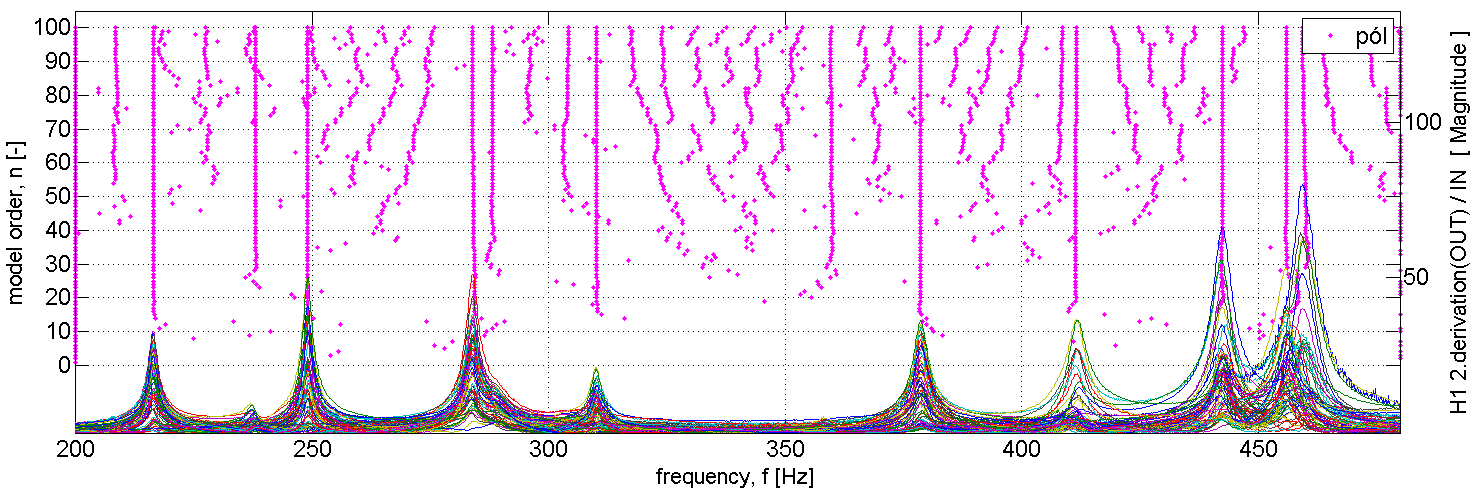
\includegraphics[width=.6\linewidth]{figs/StabilizacniDiagram.png}
		\caption{Stabilizační diagram}
	\end{figure}
	
	\section{Co je nelineární model Hammersteinova typu a nelineární model Wienerova typu. }

	Modely skládající se z dynamického lineárního přenosu $G(q)$ a statické nelineární funkce $f$
	
	\subsection*{Model Hammersteinova typu}	
	\begin{figure}[h!]
		\centering
		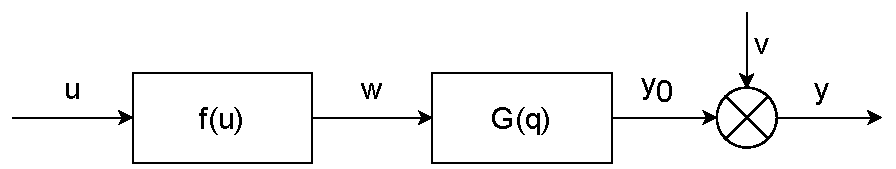
\includegraphics[width=.6\linewidth]{figs/HammersteinuvModel.pdf}
	\end{figure}
	
	\subsection*{Model Weinerova typu}	
	\begin{figure}[h!]
		\centering
		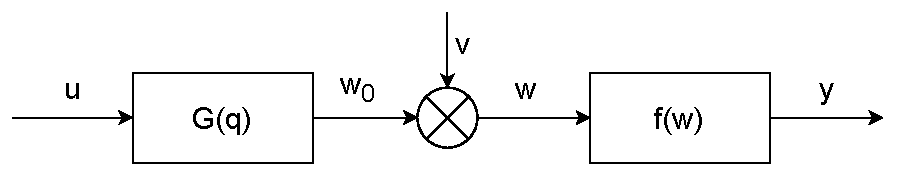
\includegraphics[width=.6\linewidth]{figs/WeineruvModel.pdf}
	\end{figure}

	\section{Uveďte strukturu nelineární identifikace používající koncept LOLIMOT. } \label{lolimot}
	\emph{LOcal LInear MOdels Tree} \\
	The main idea is to approximate
	a generally nonlinear multivariable function describing
	a dynamic system output with the scalar product of
	the vector of linear functions of the system inputs and the vector of so-called validity functions.
	\begin{equation}
		\hat{y} = \sum_{i=1}^M \hat{y}_i(\bm{x}) \phi_i(\bm{z	})
	\end{equation}
	kde $\hat{y}_i$ jsou \emph{lokální lineární modely}
	\begin{equation}
		\hat{y}_i = w_{i0} + w_{i1} x_1 + w_{i2} x_2 + \dots + w_{in}x_n
	\end{equation}
	a $\phi_i(u)$ jejich platnostní funkce, formulovány jako normalizované ortogonální Gaussovské rozdělení, které splňují
	\begin{equation}
		\sum_{i=1}^n \phi_i(u) = 1
		\;,\quad 
		\phi_i(u) = \frac{\mu_i(u)}{\sum_{i=1}^n \mu_i(u)}
		\;,\quad 
		\mu_i = \exp\left(-\frac{1}{2}\sum_{j=1}^{M}\frac{(u_j-c_{ij})^2}{\sigma_{ij}^2}\right)
	\end{equation}

	kde $M$ je počet LLM a $c_{ij}$ a $\sigma^2_{ij}$, která jsou volitelná, jsou popořadě střední hodnota a rozptyl $i$-tého rozdělení pro $j$-tý LLM. Vektory zobecněných vstupů, neboli \emph{regresorů}, $\bm{x}$ a $\bm{z}$ obecně obsahují okamžité vstupy systému $u_j(k)$, minulé vstupy systému $u_j(k-r)$ a minulé výstupy systému $y(k-s)$, kde $r$ a $s$ jsou horizonty závislosti na vstupech a výstupech, popořadě. $\bm{z}$ je nazýván vektor premis (premises) a $\bm{x}$ vektor konsekventů (consequents).

	\begin{itemize}
	\item Vnitřní cyklus: výpočet koeficientů $w_i$ LLM při daném rozložení platnostních funkcí (exaktní - LSQ)
	\item Vnější cyklus: hledání vhodného ``rozdělení'' oblasti (heuristika)
	\end{itemize}

	\section{Uveďte postup identifikace nelineárního diskrétního dynamického modelu LOLIMOT typu NARX. }

	LOLIMOT typu NARX (Nonlinear Auto Regressive with Exogenous inputs) aproximuje obecnou nelineární závislost modelu NARX pomocí lineární kombinace lokálních lineárních ARX modelů.
	\begin{equation}
		\hat{y}(t) + a_1 y(t-\Delta t) + \dots + a_n y(t-n\Delta t)
		=
		b_0 u(t) + \dots + b_n u(t-n\Delta t)
	\end{equation}
	NARX LOLIMOT lze pak zapsat jako
	\begin{equation}
		\hat{y} = \sum_{i=1}^M \bm{w}_i^T \bm{x} \phi_i(\bm{z})
		\;,\quad 
		\bm{w}_i = \begin{bmatrix} -a_{1_i} & \dots & -a_{n_i} & b_{0_i} & \dots & b_{n_i} \end{bmatrix}^T
	\end{equation}
	\pagebreak
	pro který identifikace probíhá metodou nejmenších čtverců dle schématu
	\begin{equation}
		\bm{\hat{y}} = \bm{X}\bm{W}
		\;,\quad 
		\bm{X}
		=
		\begin{bmatrix}
			\bm{x}_1 & \dots & \bm{x}_M
		\end{bmatrix}
		\,,\;
		\bm{W}
		=
		\begin{bmatrix}
		\bm{w}_1 \\ \vdots \\ \bm{w}_M
		\end{bmatrix}
	\end{equation}
	kde
	\begin{equation}
		\bm{X}_i
		=
		\begin{bmatrix}
			y_{n-1} & \dots & y_0 & u_n & \dots & u_0 \\
			\vdots & \ddots & \vdots & \vdots & \ddots & \vdots \\
			y_{N-1} & \dots & y_{N-n} & u_N & \dots & u_{N-n}
		\end{bmatrix}
		\bm{\phi}_i(\bm{z})
	\end{equation}
	Váhy jsou z něj získány pomocí pseudoinverze
	\begin{equation}
	\bm{W} = \bm{X}^+ \bm{\hat{y}}
	\end{equation}

	The basic algorithm of the identification procedure is as follows:
	\begin{enumerate}
	\item Determine the data region. Construct the validity
	function for this single global linear model equal
	to one. Construct the linear model (i.e., estimate
	its coefficients). Set the number of LLMs, M=1.
	\item Find the worst performing LLM and denote its
	index as I.
	\item The I-th LLM is considered for further
	refinement. The corresponding hyper-rectangle
	is split into two halves with an axis-orthogonal
	split. Division in each dimension dim=1...p is
	tried and the following steps are performed:
	\item Construction of all validity functions as a
	normalized orthogonal Gaussian
	functions.
	\item Estimation of parameters of both newly
	constructed LLMs (LSQ method).
	\item Calculation of the loss function for the
	current overall model (prediction or simulation error).
	\item Adopt the best of the p alternatives from the
	Step 3. Put M=M+1.
	\item Check whether the termination criterion is met; if
	so, stop the algorithm, else continue with Step 2.
	\end{enumerate}

	\begin{figure}[h!]
		\centering
		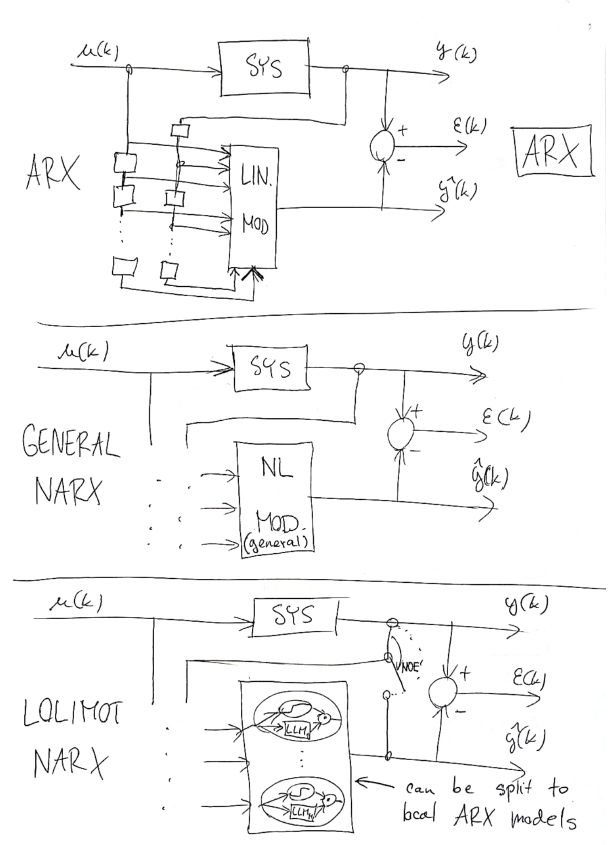
\includegraphics[width=.4\linewidth]{figs/lolimot_narx.png}
	\end{figure}

	\section{Vysvětlete pojmy testování a trénování identifikovaného modelu.}

	\subsection*{Trénování}
	Při trénování jsou parametry identifikovaného modelu upravovány tak, aby chování systému co nejvíce odpovídalo \emph{trénovacím datům}.

	\subsection*{Testování}
	Při testování porovnáváme chování identifikovaného modelu k nové sadě \emph{testovacích dat}, abychom ověřili, že nedošlo k přetrénovaní modelu, tzn. přizpůsobení ke konkrétním trénovacím datům, nikoliv obecnému chování.

	\section{Vysvětlete rozdíl mezi simulačním a predikčním trénováním a použitím LOLIMOT modelu a souvislost těchto pojmů s NARX a NOE modely. }

	\subsection*{Simulační trénování}
	Identifikovaný model je odpojený od reálného systému a pracuje pouze s jeho vstupy, kde chyba výstupu se kumuluje.

	Odpovídá schématu NOE (Nonlinear Output Error)
	\begin{equation}
		\hat{y}_k = f(u_k,u_{k-1},\dots,\hat{y}_{k-1},\hat{y}_{k-2},\dots)
	\end{equation}

	\subsection*{Predikční trénování}
	Model je připojen k výstupům modelu realného systému

	Odpovídá schématu NARX
	\begin{equation}
		\hat{y}_k = f(u_k,u_{k-1},\dots,y_{k-1},y_{k-2},\dots)
	\end{equation}

	\section{Uveďte příklad identifikace ad-hoc sestaveného dynamického modelu soustavy s pomocí obecných optimalizačních metod. }

	\section{Uveďte základní postup identifikace fyzikálního modelu získaného např. z MKP po transformaci do redukovaného modálního tvaru. V čem tato redukce usnadní postup identifikace ? }
	
	Na základě naměřených/navržených vlastností materiálu vytvořím mkp model ve tvaru
	\begin{equation*}
		\bm{M}\bm{\ddot{x}} + \bm{C}\bm{\dot{x}} + \bm{K}\bm{x} = \bm{F}
	\end{equation*}
	Ten následně transformuju do modálních souřadnic
	\begin{equation*}
		\bm{I}\bm{\ddot{q}} + \bm{\Gamma}\bm{\dot{q}} + \bm{\Omega}^2 \bm{q} = \bm{V}^T \bm{F}
		\;,\quad 
		\bm{\Omega} = \bm{V}^T\bm{K}\bm{V}
		\,,\;
		\bm{\Gamma} = \bm{V}^T\bm{B}\bm{V}
	\end{equation*}
	a oříznu mimodiagonální prvky transformované matice tlumení $\bm{\Gamma}$, přičemž prvky na diagonále lze vyjádřit jako $\beta_{ii} = 2 b_{r_i} \Omega_i$. Dále můžu provést redukci, ostraněním tvarů odpovídajících vyšším frekvencím systému.

	Vyslédkem je model závislý pouze na parametrech $\omega_i$, $b_{r_i}$ 	pro každý zanechaný tvar, které můžu dále optimalizovat. Oproti black-box identifikaci nehrozí vznik umělých artefaktů.

	\section{Uveďte příklad využití fenomenologického identifikovaného modelu pro simulaci. }
	
	Fenomenologicky například inentifikujeme tření (LuGre, Coulomb, Streibeck, ...)
	\begin{figure*}[ht!]
		\begin{subfigure}[h!]{.49\textwidth}
			\centering
			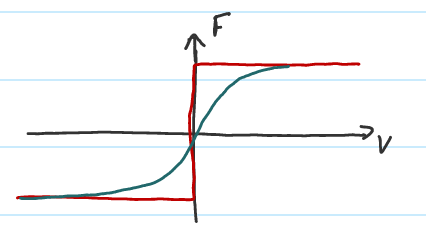
\includegraphics[width=\linewidth]{figs/Coulomb.png}
			\caption{Coulomb}
		\end{subfigure}
		\hfill
		\begin{subfigure}[h!]{.49\textwidth}
			\centering
			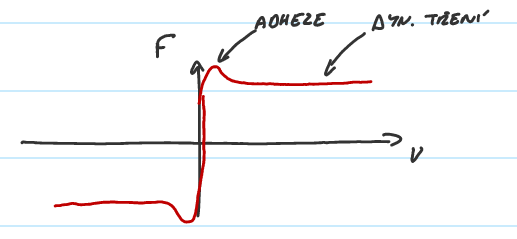
\includegraphics[width=\linewidth]{figs/Streibeck.png}
			\caption{Streibeck}
		\end{subfigure}
	\end{figure*}
	nebo nelineární chování tlumiče.

	\section{Popište použití identifikovaného modelu soustavy v regulátoru s prediktivním řízením. Jak souvisí s pojmy NARX a NOE modelů ? }

	\begin{align}
		\bm{x}_{k+1} &= \bm{A}\bm{x}_k + \bm{B}\bm{u}_k \\
		\bm{y}_k &= \bm{C}\bm{x}_k
	\end{align}

	\begin{align}
		\bm{\hat{x}}_{k+1} &= \bm{A}\bm{x}_k + \bm{B}\bm{u}_k \\
		\bm{\hat{x}}_{k+2} &= \bm{A}^2\bm{x}_k + \bm{A}\bm{B}\bm{u}_k + \bm{B}\bm{u}_{k+1}\\
		\bm{\hat{x}}_{k+n} &= \bm{A}^n\bm{x}_k + \sum_{i=1}^n \bm{A}^{n-i}\bm{B}\bm{u}_{k+i-1}
	\end{align}

	\begin{equation}
		\bm{\hat{y}}_{k+n} = \bm{C}\bm{A}^n\bm{x}_k + \sum_{i=1}^n \bm{C}\bm{A}^{n-i}\bm{B}\bm{u}_{k+i}
	\end{equation}

	\begin{equation}
		\bm{\hat{Y}} = \bm{f} + \bm{G}\bm{U}
	\end{equation}
	\begin{equation}
		\bm{\hat{Y}}
		=
		\begin{bmatrix}
			\bm{\hat{y}}_{k+1} \\
			\vdots \\
			\bm{\hat{y}}_{k+N}
		\end{bmatrix}
		\;,\quad 
		\bm{f}
		=
		\begin{bmatrix}
			\bm{C}\bm{A} \\
			\vdots \\
			\bm{C}\bm{A}^N
		\end{bmatrix}
		\bm{x}_k
		\;,\quad 
		\bm{G}
		=
		\begin{bmatrix}
			\bm{C}\bm{B} &  & \bm{0} \\
			\vdots & \ddots & \\
			\bm{C}\bm{A}^{N-1}\bm{B} & \dots & \bm{C}\bm{B}
		\end{bmatrix}
		\;,\quad 
		\bm{U}
		=
		\begin{bmatrix}
			\bm{u}_{k} \\
			\vdots \\
			\bm{u}_{k+N-1}
		\end{bmatrix}
	\end{equation}

	\begin{align}
	\bm{J}_k &= (\bm{\hat{Y}}-\bm{W})^T \bm{Q} (\bm{\hat{Y}}-\bm{W}) + \bm{U}^T\bm{P}\bm{U} = (\bm{f+GU}-\bm{W})^T \bm{Q} (\bm{f+GU}-\bm{W}) + \bm{U}^T\bm{P}\bm{U} \\
	\frac{\partial\bm{J}_k}{\partial\bm{U}} &= 2(\bm{f-W})^T\bm{QG}+2\bm{U}^T(\bm{G^TQG+P}) = 0 \\
	\bm{U} &= \bm{(G^TQG+P)^{-1} G^T Q (f-W)}
	\end{align}
% \end{multicols}
\end{document}